% Results
\subsection{Environment and Actions}
In the discrete representation of our Parking Mesh environment, the continuous nature of a city—such as Madrid, which spans roughly 604.3~km² (604,300,000~m²)—is discretized into grid squares of 6~meters by 6~meters (36~m²). This results in approximately 16.8 million squares (\(604,300,000 \div 36\)) to represent the full city.

Each square represents a discrete state-space unit with properties such as:
\begin{itemize}
    \item \textbf{Occupancy status} (vacant or occupied),
    \item \textbf{Pricing information},
    \item \textbf{Zone classification} (residential, commercial, etc.).
\end{itemize}

These attributes are pre-established in coordination with local administrations.

\subsubsection*{Partially Observable State}\leavevmode

Each vehicle (agent) perceives only a local neighborhood of cells (e.g., a 3×3 or 5×5 grid centered on itself). For each visible cell, the agent’s state vector includes:
\begin{itemize}
    \item \textbf{Occupancy Status:} Derived from onboard sensors.
    \item \textbf{Cell Metadata:} Zone type, hourly rate, max parking duration.
    \item \textbf{Neighbor Communications:} Broadcast updates from nearby agents over Bluetooth mesh.
\end{itemize}

\begin{figure}[H]
    \centering
    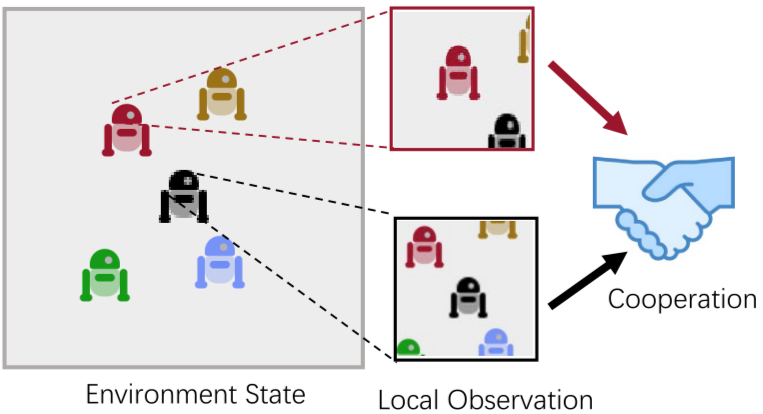
\includegraphics[width=0.8\linewidth]{Figures/partial_observation.png}
    \captionsetup{justification=centering}
    \caption{Partially observable state space for local agents.\footcite{moonlightMARL}}
    \label{fig:partial-observability}
\end{figure}
\footnotetext[7]{Adapted from \cite{moonlightMARL}.}
\subsubsection*{Agent Actions}\leavevmode

At each timestep, agents choose from a discrete action set:
\begin{itemize}
    \item \textbf{Detect Vacancy/Occupancy:} Use sensors (e.g., ultrasonic, camera) to scan adjacent cells.
    \item \textbf{Broadcast Update:} Transmit new occupancy/vacancy findings to nearby agents.
    \item \textbf{Relay Message:} Forward information from others to expand knowledge range.
    \item \textbf{Query Neighbors:} Request occupancy data for specific cells when local knowledge is outdated.
\end{itemize}

\subsubsection*{Multi-Agent Reinforcement Learning (MARL)}\leavevmode

\vspace{0.5em}
The Parking Mesh problem naturally maps onto a Multi-Agent Reinforcement Learning (MARL) framework. Each equipped vehicle functions as an autonomous agent, responsible for sensing local parking availability and sharing that information. Since efficient parking management depends on collective knowledge rather than isolated behavior, a cooperative MARL setup is ideal. In this setting, agents are not in competition but instead support one another by enhancing local awareness—ultimately reducing search times, easing congestion, and cutting emissions.

This collaborative structure allows the network as a whole to outperform isolated decision-making by maximizing shared objectives, such as minimizing drivers' parking time and improving urban traffic flow. Furthermore, the underlying architecture of the Parking Mesh—vehicles as nodes connected via short-range Bluetooth communication—lends itself naturally to a Graph Neural Network (GNN) implementation. GNNs are well-suited for modeling such relational data, as they propagate observations through network connections and capture inter-agent dynamics. By representing vehicles as graph nodes and their communication links as edges, GNNs enable the system to learn coordinated parking strategies that fully exploit the spatial and communicative structure of the mesh network.
